%%%%%%%%%%%%%%%%%%%%%%%%%%%%%%%%%%%%%%%%%%%%%%%%%%%%%%%%%%%%%%%%%%%%%%%%%%%%%%%%%%%
%% This project aims to create the UFC template for presentation.                %%
%% author: Maurício Moreira Neto - Doctoral student in Computer Science (MDCC)   %%
%% contacts:                                                                     %%
%%    e-mail: maumneto@ufc.br                                                    %%
%%    linktree: https://linktr.ee/maumneto                                       %%
%%%%%%%%%%%%%%%%%%%%%%%%%%%%%%%%%%%%%%%%%%%%%%%%%%%%%%%%%%%%%%%%%%%%%%%%%%%%%%%%%%%
\documentclass{libs/ufc_format}
% Inserting the preamble file with the packages
%%%%%%%%%%%%%%%%%%%%%%%%%%%%%%%%%%%%%%%%%%%%%%%%%%%%%%%%%%%%%%%%%%%%%
%% This file contains the packages that can be used in the beamer. %%
%%%%%%%%%%%%%%%%%%%%%%%%%%%%%%%%%%%%%%%%%%%%%%%%%%%%%%%%%%%%%%%%%%%%%
% Package to fonts family
\usepackage[T1]{fontenc}
% Package to accentuation
\usepackage[utf8]{inputenc}
% Package to Portuguese language
\usepackage[brazil]{babel}
% Package to Figures
\usepackage{graphicx}
% Package to the colors
\usepackage{color}
% Package to the colors
\usepackage{xcolor}
% Packages to math symbols and expressions
\usepackage{amsfonts, amssymb, amsmath}
% Package to multiple lines and columns in table
\usepackage{multirow, array} 
% Package to create pseudo-code
% For more detail of this package: http://linorg.usp.br/CTAN/macros/latex/contrib/algorithm2e/doc/algorithm2e.pdf
\usepackage{algorithm2e}
% Package to insert code
\usepackage{listings} 
\usepackage{keyval}
% Package to justify text
\usepackage[document]{ragged2e}
% Package to manage the bibliography
\usepackage[backend=biber, style=numeric, sorting=none]{biblatex}
% Package to facilities quotations
\usepackage{csquotes}
% Package to use multicols
\usepackage{multicol}

% Packages added by me
\usepackage{url}
\usepackage{tikz}
%\usepackage{multimedia}
%\usepackage{media9}[playbutton=plain, windowed=1280x720]
% Inserting the references file
\bibliography{references.bib}
\renewcommand*{\bibfont}{\scriptsize}

% Title
\title[Introdução a IA]{\huge\textbf{Introdução à Inteligência Artificial}}
% Subtitle
\subtitle{Parte 3}
% Author of the presentation
\author{Evandro J.R. Silva}
% Institute's Name
\institute[Estácio Teresina]{
    % email for contact
    \normalsize{\email{ejrs.profissional@gmail.com}}
    \newline
    % Department Name
    %\department{Bacharelado em Ciência da Computação}
    \newline
    % university name
    %\ufc
    \estaciothe
}
% date of the presentation
\date{30 e 31 de Janeiro}


%%%%%%%%%%%%%%%%%%%%%%%%%%%%%%%%%%%%%%%%%%%%%%%%%%%%%%%%%%%%%%%%%%%%%%%%%%%%%%%%%%
%% Start Document of the Presentation                                           %%               
%%%%%%%%%%%%%%%%%%%%%%%%%%%%%%%%%%%%%%%%%%%%%%%%%%%%%%%%%%%%%%%%%%%%%%%%%%%%%%%%%%
\begin{document}
% insert the code style
%%%%%%%%%%%%%%%%%%%%%%%%%%%%%%%%%%%%%%%%%%%%%%%%%%%%%%%%%%%%%%%%%%%%%%%%%%%%%%%%%%%
%% This file contains the style of the codes show in slides.                     %%
%% The package used is listings, but it possible to used others.                 %%
%%%%%%%%%%%%%%%%%%%%%%%%%%%%%%%%%%%%%%%%%%%%%%%%%%%%%%%%%%%%%%%%%%%%%%%%%%%%%%%%%%%

% color used in the code style
\definecolor{codegreen}{rgb}{0,0.6,0}
\definecolor{codegray}{rgb}{0.5,0.5,0.5}
\definecolor{codepurple}{rgb}{0.58,0,0.82}
\definecolor{codebackground}{rgb}{0.95,0.95,0.92}

% style of the code!
\lstdefinestyle{codestyle}{
    backgroundcolor=\color{codebackground},   
    commentstyle=\color{codegreen},
    keywordstyle=\color{magenta},
    numberstyle=\tiny\color{codegray},
    stringstyle=\color{codepurple},
    basicstyle=\ttfamily\footnotesize,
    frame=single,
    breakatwhitespace=false,         
    breaklines=true,                 
    captionpos=b,                    
    keepspaces=true,                 
    numbers=left,                    
    numbersep=5pt,                  
    showspaces=false,                
    showstringspaces=false,
    showtabs=false,                  
    tabsize=2,
    title=\lstname 
}

\lstset{style=codestyle}


%% ---------------------------------------------------------------------------
% First frame (with tile, subtitle, ...)
\begin{frame}{}
    \maketitle
\end{frame}

%% ---------------------------------------------------------------------------
% Second frame
\begin{frame}{Sumário}
    \begin{multicols}{2}
        \tableofcontents
    \end{multicols}
\end{frame}

%=============================================================================
% SECTION 1
%=============================================================================
\section{Resolução de Problemas por meio de Busca}

\begin{frame}{}
    \centering
    \Large
    Resolução de Problemas por meio de Busca
\end{frame}

\begin{frame}{Resolução de Problemas por meio de Busca}
    \begin{itemize}
        \justifying
        \item Este é o caso de um agente baseado em objetivo.
        \item Vamos começar com o tipo mais simples de ambiente de tarefa, para o qual a solução para um problema é sempre uma sequência fixa de ações.
    \end{itemize}
\end{frame}

\begin{frame}{Resolução de Problemas por meio de Busca}
    \centering
    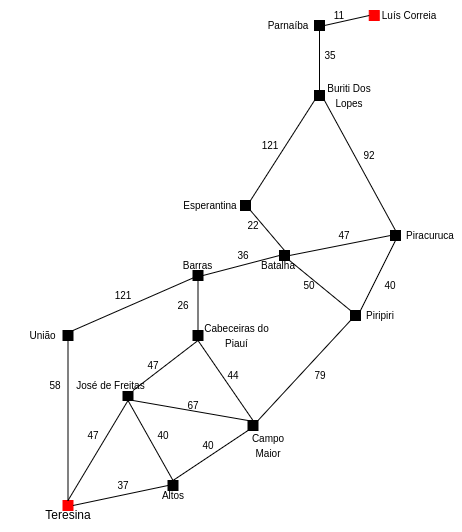
\includegraphics[width=0.65\textwidth]{figuras/problema01}
\end{frame}

\begin{frame}{Resolução de Problemas por meio de Busca}
    \begin{itemize}
        \justifying
        \item \textbf{Problema:} ir de \textbf{Teresina} para \textbf{Luís Correia}.
        \item<2-> A partir de Teresina existem 3 possibilidades. Se o ambiente for desconhecido, ou seja, se o agente não tem qualquer informação adicional, terá de escolher entre uma das três aleatoriamente.
        \item<3-> Mas vamos levar em consideração que o agente possui o mesmo mapa que vimos.
            \begin{itemize}
                \justifying
                \item<3-> Portanto o ambiente é \textbf{observável} (pois o agente sempre conhecerá o estado atual), \textbf{discreto} (pois para cada estado existe um número finito de ações a escolher), \textbf{conhecido} (agora o agente sabe quais estados serão alcançados após uma ação) e \textbf{determinístico} (pois cada ação tem exatamente um resultado).
            \end{itemize}
    \end{itemize}
\end{frame}

\begin{frame}{Resolução de Problemas por meio de Busca}
    \begin{itemize}
        \justifying
        \item Temos
            \begin{itemize}
                \justifying
                \item \textbf{Estado Inicial}: Está em Teresina.
                \item \textbf{Objetivo}: Estar em Luís Correia.
                \item \textbf{Ações}: Ir para alguma cidade.
                \item \textbf{Espaço de estados}: todos os estados acessíveis a partir do estado inicial.
                \item \textbf{Teste de objetivo}: Estamos em Luís Correia?
            \end{itemize}
        \item<2-> Custo de caminho: quanto ``custa'' acrescentar um determinado estado? E como calcular esse custo?
    \end{itemize}
\end{frame}

\begin{frame}{Resolução de Problemas por meio de Busca}
\centering
    Breve exemplificação com outro problema:\\
    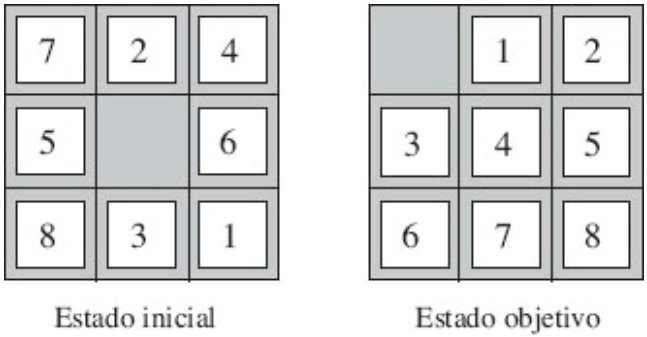
\includegraphics[width=0.5\textwidth]{figuras/figura09}
    \begin{itemize}
        \scriptsize
        \justifying
        \item<1-3> \textbf{Estados:} Uma descrição de estado especifica a posição de cada uma das oito peças e do quadrado vazio em um dos nove quadrados.
        \item<2-4> \textbf{Estado inicial:} O que está na figura, porém qualquer estado pode ser designado como o estado inicial.
        \item<3-5> \textbf{Ações:} A formulação mais simples define as ações como movimentos do quadrado vazio, \textit{Esquerda}, \textit{Direita}, \textit{Para Cima} ou \textit{Para Baixo}.
        \item<4-6> \textbf{Modelo de Transição:} (não pode ser esquecido enquanto você estiver produzindo o programa de agente) Dado um estado e ação, ele devolve o estado resultante; por exemplo, se aplicarmos \textit{Esquerda} para o estado inicial na figura, o estado resultante terá comutado o 5 e o branco.
        \item<5-> \textbf{Teste de objetivo:} Verifica se o estado corresponde à configuração de estado objetivo mostrada na figura.
        \item<6> \textbf{Custo de caminho:} Cada passo custa 1 e,assim, o custo do caminho é o número de passos do caminho.
    \end{itemize}
\end{frame}

%----------------------------------------------------------------------------
% SUBSECTION 1.1
%----------------------------------------------------------------------------
\subsection{Estratégias de Busca}

\begin{frame}{Estratégias de Busca}
    \begin{itemize}
        \item Voltemos ao nosso problema original!
    \end{itemize}
    \centering
    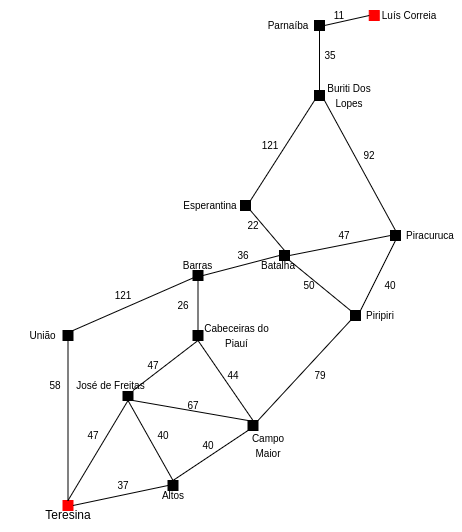
\includegraphics[width=0.55\textwidth]{figuras/problema01}
\end{frame}

\begin{frame}{Estratégias de Busca}
    \begin{itemize}
        \justifying
        \item Como se trata de um grafo, podemos utilizar uma busca em árvore (atenção que eu vou desenhar no quadro).
        \item<2-> Como fazer para não repetir um estado?
        \item<3-> Como construir o caminho?
            \begin{itemize}
                \item<4> \textbf{Busca em Largura}\\
                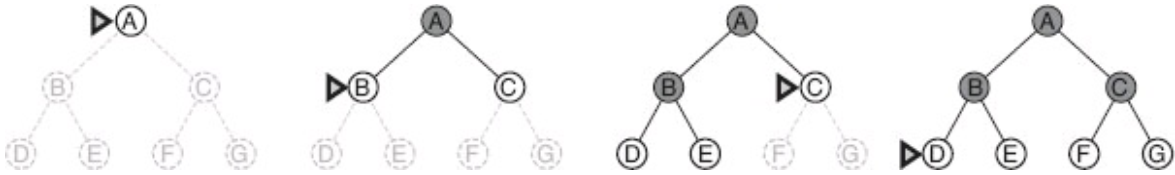
\includegraphics[width=0.85\textwidth]{figuras/figura10}
                \item<4> \textbf{Busca de custo uniforme}: em vez de expandir o nó mais raso, é expandido o nó com o menor custo de caminho.
                \item<4> \textbf{Busca em Profundidade}, a qual pode ser modificada para busca com profundidade limitada e aprofundamente iterativo.
            \end{itemize}
    \end{itemize}
\end{frame}

%=============================================================================
% SECTION 2
%=============================================================================
\section{Busca com Informação}

\begin{frame}{}
    \centering
    \Large
    Busca com Informação
\end{frame}

\begin{frame}{Busca com Informação (Heurística)}
    \begin{itemize}
        \justifying
        \item Com a adição de informação, podemos melhorar nossa estratégia de busca, através da adição de uma \textbf{função de avaliação} --- ou seja, uma forma de medir o quão boa é uma determinada solução.
        \item<2> Utilizando o nosso exemplo, vamos levar em consideração que agora sabemos a distância \alert{em linha reta} entre cada cidade e o destino que queremos alcançar. Então teremos a seguinte tabela:\\
        \begin{table}[]
            \centering
            \begin{tabular}{|l|l||l|l|}
            \hline
                Teresina & 277              &   Esperantina & 129 \\
                Altos & 255                 &   Batalha & 134 \\
                União & 231                 &   Piripiri & 155 \\
                José de Freitas & 231       &   Piracuruca & 117 \\
                Barras & 167                &   Buriti dos Lopes & 40 \\
                Cabeceiras do Piauí & 191   &   Parnaíba & 10 \\
                Campo Maior & 223           &   Luís Correia & 0\\
                \hline
            \end{tabular}
            \caption{Distância em linha reta para Luís Correia}
            \label{tab:my_label}
        \end{table}
    \end{itemize}
\end{frame}

%----------------------------------------------------------------------------
% SUBSECTION 2.1
%----------------------------------------------------------------------------
\subsection{Busca Gulosa}

\begin{frame}{Busca Gulosa, ou \textit{Greed Search}}
    \begin{itemize}
        \justifying
        \item O algoritmo \textbf{Busca Gulosa} procura pelo ``vizinho mais próximo''.
    \end{itemize}
\end{frame}

\begin{frame}{Busca Gulosa, ou \textit{Greed Search}}
    \centering
    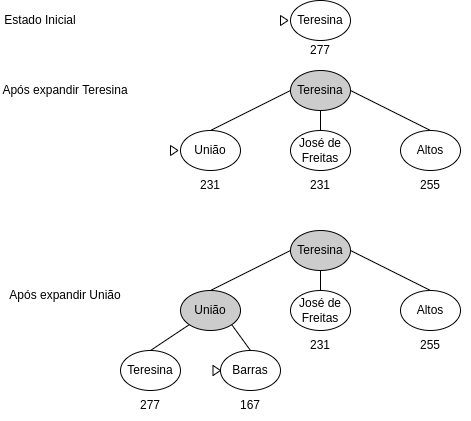
\includegraphics[width=0.75\textwidth]{figuras/guloso}
\end{frame}

\begin{frame}{Busca Gulosa, ou \textit{Greed Search}}
    \begin{itemize}
        \justifying
        \item A continuação seria:
            \begin{itemize}
                \justifying
                \item Barras $\rightarrow$ Batalha $\rightarrow$ Piracuruca $\rightarrow$ Buriti dos Lopes $\rightarrow$ Parnaíba $\rightarrow$ Luís Correia.
            \end{itemize}
        \item A distância total (a partir de Teresina): 58 + 121 + 36 + 47 + 92 + 35 + 11 = 400km.
        \item<2-> É o caminho mais curto?
        \item<3-> É possível que não! Vamos testar outro algoritmo.
    \end{itemize}
\end{frame}

%----------------------------------------------------------------------------
% SUBSECTION 2.2
%----------------------------------------------------------------------------
\subsection{Busca A*}

\begin{frame}{A*}
    \begin{itemize}
        \justifying
        \item Este algoritmo (\textit{a estrela}) utiliza, além do conhecimento que adquirimos, o custo para se alcançar cada estado.
    \end{itemize}
    \centering
    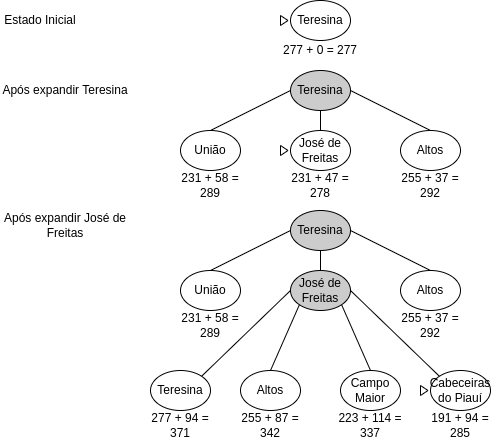
\includegraphics[width=0.7\textwidth]{figuras/a_estrela}
\end{frame}

\begin{frame}{A*}
    \begin{itemize}
        \justifying
        \item É possível que o A* demore mais para encontrar uma solução em relação ao Algoritmo Guloso, porém é garantido que a solução será a melhor.
        \item<2-> Numa situação de ``mundo real'', pode acontecer do A* demorar muito, muito mesmo, devido à quantidade de estados possíveis.
        \item<3-> Por causa disso existem outros algoritmos de busca, os quais são modificações ou inspirados no A*: IDA* (\textit{Iterative Deepening A*} --- Aprofundamento Iterativo A*) e RBFS (\textit{Recursive Best First Search} --- Busca Recursiva de Melhor Escolha).
        \item<4-> \alert{Tarefa de casa: pesquisar sobre esses e outros algoritmos!}
    \end{itemize}
\end{frame}
%=============================================================================
% SECTION ?
%=============================================================================
\section{FIM}

\begin{frame}{}
    \centering
    \Large
    Terminamos a Terceira Parte!\\
    Obrigado pela atenção!
\end{frame}

%=============================================================================
% SECTION REFERENCES
%=============================================================================
%\begin{frame}[allowframebreaks]{Referências}
%    \scriptsize
%    \printbibliography
%\end{frame}

\end{document}













%% ---------------------------------------------------------------------------
% This presentation is separated by sections and subsections
%\section{Seção I}
%\begin{frame}{Explicações}
%    % itemize
%    Este é um template que pode ser utilizado para:
%    \begin{itemize}
%        \item Apresentação de Trabalhos Acadêmicos
%        \item Apresentação de Disciplinas
%        \item Apresentações de Teses e Dissertações
%    \end{itemize}
%
%    \vspace{0.4cm} % vertical space
%    
%    % enumeration
%    Para utilizar este template corretamente é importante que:
%    \begin{enumerate}
%        \item Tenha conhecimento mínimo sobre LaTeX
%        \item Ler os comentários no template (explicações)
%        \item Ler o README.md (documentação)
%    \end{enumerate}
%
%    \vspace{0.2cm}

%    \example{Este é um texto de exemplo!} \emph{Texto de Ênfase!}
%\end{frame}

%% ---------------------------------------------------------------------------
%\subsection{Subseção I}
%\begin{frame}{Criando Blocos}
%    % Blocks styles
%    \begin{block}{Bloco Padrão}
%        Texto do corpo do bloco.
%    \end{block}

%    \begin{alertblock}{Bloco de Alerta}
%        Texto do corpo do bloco.
%    \end{alertblock}
%
%    \begin{exampleblock}{Bloco de Exemplo}
%        Texto do corpo do bloco.
%    \end{exampleblock}   
%\end{frame}

%% ---------------------------------------------------------------------------
%\subsection{Subseção II}
%\begin{frame}{Criando Caixas}
%    \successbox{testando o success box}
%
%    \pause
%
%    \alertbox{testando o alert box}
%
%    \pause
%
%    \simplebox{testando o simple box}
%\end{frame}

%% ---------------------------------------------------------------------------
%\subsection{Subseção III}
%\begin{frame}{Criando Algoritmos (Pseudocódigo)}
%    \begin{algorithm}[H]
%        \SetAlgoLined
%        \LinesNumbered
%        \SetKwInOut{Input}{input}
%        \SetKwInOut{Output}{output}
%        \Input{x: float, y: float}
%        \Output{r: float}
%        \While{True}{
%          r = x + y\;
%          \eIf{r >= 30}{
%           ``O valor de $r$ é maior ou iqual a 10.''\;
%           break\;
%           }{
%           ``O valor de $r$ = '', r\;
%          }
%         } 
%         \caption{Algorithm Example}
%    \end{algorithm}
%\end{frame}

%% ---------------------------------------------------------------------------

%\begin{frame}{Inserindo Algoritmos}
%    \lstset{language=Python}
%    \lstinputlisting[language=Python]{code/main.py}
%\end{frame}

%% ---------------------------------------------------------------------------
%\begin{frame}{Inserindo Algoritmos}
%    \lstinputlisting[language=C]{code/source.c}
%\end{frame}

%% ---------------------------------------------------------------------------
%\begin{frame}{Inserindo Algoritmos}
%    \lstinputlisting[language=Java]{code/helloworld.java}
%\end{frame}

%% ---------------------------------------------------------------------------
%\begin{frame}{Inserindo Algoritmos}
%    \lstinputlisting[language=HTML]{code/index.html}
%\end{frame}

%% ---------------------------------------------------------------------------
% This frame show an example to insert multicolumns
%\section{Multicolunas}
%\begin{frame}{Seção II - Multicolunas}
%    \begin{columns}{}
%        \begin{column}{0.5\textwidth}
%            \justify
%            É possível colocar mais de uma coluna utilizando os comandos de $\backslash$begin\{column\}\{\} e $\backslash$end\{column\}
%        \end{column}
%        \begin{column}{0.5\textwidth}
%            \justify
%            Porém, o espaçamento deve ser proporcional entre as colunas para que estas colunas não entrem em coflito. O espaçamento é dado pelo segundo argumento do $\backslash$begin.
%        \end{column}
%    \end{columns}    
%\end{frame}

%% ---------------------------------------------------------------------------
% This frame show an example to insert figures
%\section{Imagens}
%\begin{frame}{Seção III - Figures}
%    \begin{figure}
%        \centering
%        \caption{Emblema da UFC.}
%        
\includegraphics[scale=0.3]{libs/emblemufc.pdf}
%        \source{Obtido pelo site oficial da UFC \cite{siteufc} \cite{einstein}}
%        \label{fig:ufc_emblem}
%    \end{figure}
%\end{frame}

%% ---------------------------------------------------------------------------
% Reference frames
%\begin{frame}[allowframebreaks]
%    \frametitle{Referências}
%    \printbibliography
%\end{frame}

%% ---------------------------------------------------------------------------
% Final frame
%\begin{frame}{}
%    \centering
%    \huge{\textbf{\example{Obrigado(a) pela Atenção!}}}
%    
%    \vspace{1cm}
%    
%    \Large{\textbf{Contato:}}
%    \newline
%    \vspace*{0.5cm}
%    \large{\email{usuario@dominio}}
%\end{frame}